\documentclass[11pt, letterpaper]{article}
\usepackage[utf8]{inputenc}
\usepackage{amsmath, amssymb}
\usepackage{geometry}
\geometry{margin=0.75in}
\usepackage{graphicx}
\usepackage{float}
\usepackage{caption}
\usepackage{siunitx}
\usepackage{booktabs}

\title{Programming Assignment 3}
\author{by Paz Lieghton}
\date{\small Applied Probability and Statistics. Prof. Lucas Finazzi}

\begin{document}
	\maketitle
	
	\section*{Introduction}
	This report fits a linear model $A(x) = \hat{a}_1 + \hat{a}_2 x$ measurements $(x_i, y_i)$ with $\sigma = 0.3$ on each $y_i$. Part~A finds the best fit parameters and covariance matrix by weighted least squares and checks the fit quality with $\chi^2$. Part~B propagates uncertnties to predicted values, showing what breaks when the off diagonal covariance is ignored which is something often overlooked. Part~C runs a Monte Carlo simulation to verify the $\chi^2$ distribution. All code uses NumPy, SciPy, and Matplotlib.
	
	\section{Linear Least Squares Fit}
	
	\subsection{Parameters and Covariance}
		\begin{table}[H]
		\centering
	
		\begin{tabular}{lrrrrrrrrrrr}
			\toprule
			$x$ & 2.0 & 2.1 & 2.2 & 2.3 & 2.4 & 2.5 & 2.6 & 2.7 & 2.8 & 2.9 & 3.0 \\
			$y$ & 2.78 & 3.29 & 3.29 & 3.33 & 3.23 & 3.69 & 3.46 & 3.87 & 3.62 & 3.40 & 3.99 \\
			\bottomrule
			
		\end{tabular}
		\caption{Dataset ($\sigma = 0.3$ on all $y_i$).}
	\end{table}
	With weights $w = 1/\sigma^2$ one defines $S,\,S_x,\,S_y,\,S_{xx},\,S_{xy}$ and $\Delta = S S_{xx} - S_x^2$. The estimators from the normal equations are
	\[
	\hat{a}_1 = \frac{S_{xx}\,S_y - S_x\,S_{xy}}{\Delta}, \qquad
	\hat{a}_2 = \frac{S\,S_{xy} - S_x\,S_y}{\Delta},
	\]
	with covariance matrix $\mathrm{Cov}(\hat{a}_1,\hat{a}_2) = \tfrac{\sigma^2}{\Delta}\!\begin{pmatrix}S_{xx}&-S_x\\-S_x&S\end{pmatrix}$        Applied to Table~1:
	\[
	\hat{a}_1 = 1.45 \pm 0.721, \qquad \hat{a}_2 = 0.799 \pm 0.286, \qquad
	\mathrm{Cov}(\hat{a}_1,\hat{a}_2) = -0.205.
	\]
	

	
	The off-diagonalis $\mathrm{Cov} \propto -S_x < 0$: a larger slope forces a smaller intercept to keep the line through the data, thus the parameters are anti-correlated.
	
	%As a cross-check, the same fit was run with \texttt{scipy.odr} (\texttt{fit\_type=2}). After rescaling its output covariance by $\sigma^2$, both parameters and the full covariance matrix agree to six decimal places with the analytic result.
	
	\subsection{Goodness of Fit}
	The chi square statistic $\chi^2 = \sum_i (y_i - \hat{a}_1 - \hat{a}_2 x_i)^2/\sigma^2$ with $\nu = n - 2 = 9$ degrees of freedom gives $\chi^2 = 4.64$ and $p = 0.864$.
	
	Since $\chi^2 < \nu$, two interpretations are possible: the model is correct and this sample happened to scatter less than average (supported by $p \gg 0.05$) as discussed in class, or $\sigma = 0.3$ slightly overestimates the true uncertainty. Either way the linear model is not rejected. Setting $\sigma = 0.2$ in the code flips $\chi^2$ above $\nu$, affirming that the declared $\sigma$ is driving this flipped relation.
	
	\begin{figure}[H]
		\centering
		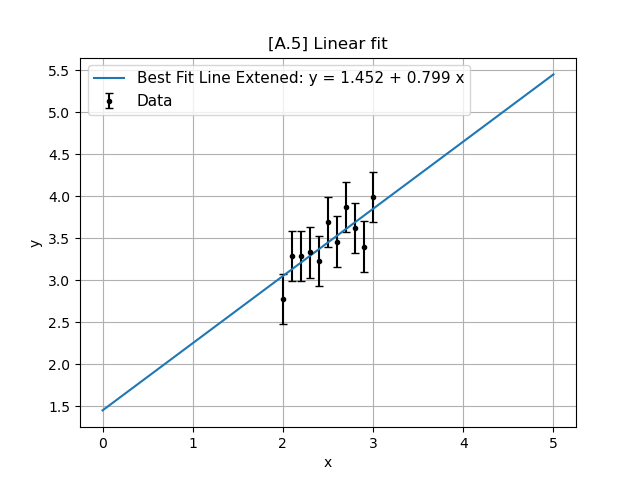
\includegraphics[width=0.65\textwidth]{fig_a5.png}
		\caption{Data with $\pm\sigma$ error bars and best-fit line $\hat{y} = 1.45 + 0.799\,x$ over $x \in [0,5]$.}
	\end{figure}
	
	\section{Uncertainty of Predicted Values and the Role of the Covariance}
	
	\subsection{Variance and Minimums}
	For a predicted value $\hat{y}_a = \hat{a}_1 + \hat{a}_2 x_a$, error propagation gives
	\[
	\mathrm{Var}(\hat{y}_a) = \sigma_{a_1}^2 + x_a^2\,\sigma_{a_2}^2 + 2x_a\,\mathrm{Cov}(\hat{a}_1,\hat{a}_2).
	\]
	The cross sterm is negative for all $x_a > 0$, so dropping it (setting $\mathrm{Cov}=0$) overestimates the uncertainty. Setting it as  $d\,\mathrm{Var}/dx_a = 0$:
	\[
	x_a^* = -\frac{\mathrm{Cov}(\hat{a}_1,\hat{a}_2)}{\sigma_{a_2}^2}
	= \frac{S_x/\Delta}{S/\Delta} = \frac{S_x}{S} = \bar{x}.
	\]
	With uniform weights $\bar{x} = 2.5$, confirmed numerically as $0.205/0.0818 = 2.5$. The line is pinned at the center and uncertainty grows as we get farther from $\bar{x}$.
	
	\begin{figure}[H]
		\centering
		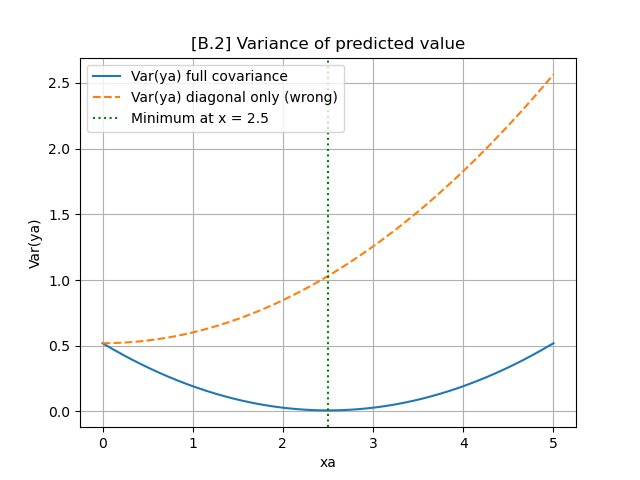
\includegraphics[width=0.65\textwidth]{fig_b2.png}
		\caption{$\mathrm{Var}(\hat{y}_a)$ vs $x_a$. Blue: full covariance (correct). Orange: diagonal only (incorrect). Green: minimum at $\bar{x} = 2.5$.}
	\end{figure}
	
	\subsection{Confidence Bands}
	Figure~3 shows the $\pm\sqrt{\mathrm{Var}(\hat{y}_a)}$ bands on the fit. The correct band (darker) is narrowest at $\bar{x}$ and widens symmetrically. The diagonal-only band (lighter) is always WIDER. The dashed line marks $\bar{y} = 3.450$, which lies on at the fit at $x = \bar{x}$ .
	
	\begin{figure}[H]
		\centering
		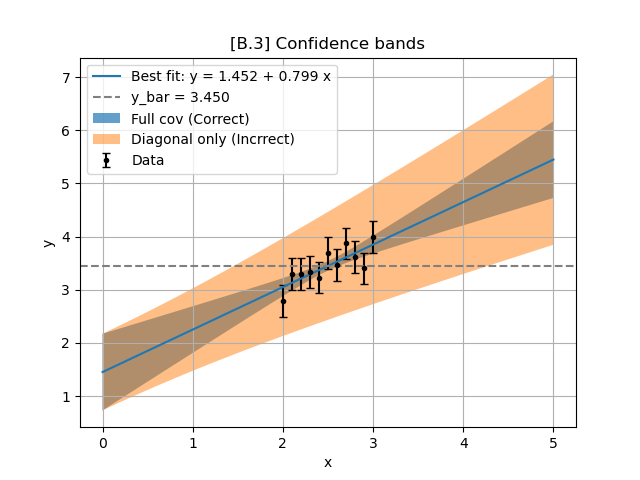
\includegraphics[width=0.65\textwidth]{fig_b3.png}
		\caption{Best fit line with corrct(darker) and diagonal(lighter) confidence bands. Dashed line its at: $\bar{y} = 3.450$.}
	\end{figure}
	
	\section{Monte Carlo Validation}
	
	$N=1000$ synthetic datasets were generated by drawing $y_i \sim \mathcal{N}(\hat{a}_1 + \hat{a}_2 x_i,\,\sigma^2)$, fitting each by least squares, and recording the $\chi^2$. The resulting histogram matches the $\chi^2(9)$ density (Figure.4), with simulated mean $8.918 \approx 9$ and std $ 4.352\approx 4.24$, confirming the analytic prediction.
	
	If the wrong model were used, the residues would inflate $\chi^2$ above $\nu$ and shift the entire histogram to the right, making the misfit immediately visible, in this case its very close.
	
	The bonus C.2 item demonstrates this: see the Appendix for the BONUS excercise, which had a great degree of effort.
	
	\begin{figure}[H]
		\centering
		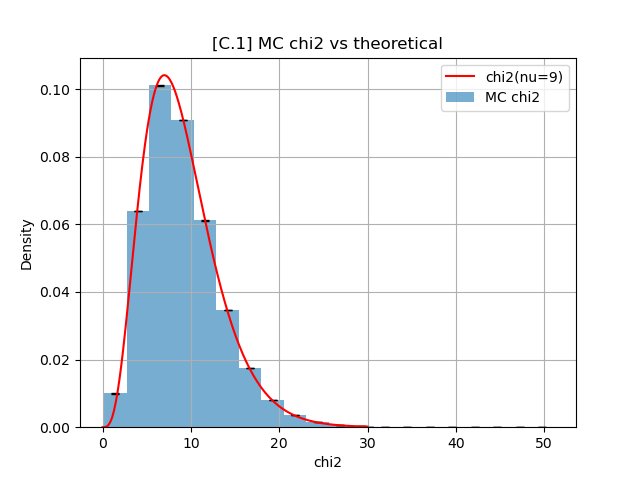
\includegraphics[width=0.65\textwidth]{fig_c1.png}
		\caption{MC $\chi^2$ histogram (1000 datasets) with Poisson errors and theoretical $\chi^2(9)$ the code sent has more bins in this same plot.}
	\end{figure}
	
	\section*{Conclusion}
	Weighted least squares gives the best-fit-line $\hat{y} = 1.45 + 0.799\,x$ with $\chi^2 = 4.64$ ($p = 0.864$), consistent with the linear model. The off diagonal covariance $-0.205$ encodes the anti correlation between intercept and slope and must be included when propagating uncertainties like the background and motivation of the assignment was: ignoring it overestimates $\mathrm{Var}(\hat{y}_a)$ everywhere, the correct variance is minimised at $\bar{x} = 2.5$.
	The Monte Carlo simulation confirms that the $\chi^2$ statistic follows $\chi^2(9)$ exactly when the model is good enough.
	
	\section*{Sources}
	\begin{itemize}
		\item Cowan, Glen. \textit{Statistical Data Analysis in Particle Physics}. Oxford University Press, 1998.
		\item SciPy Documentation. \texttt{scipy.odr} module. \texttt{https://docs.scipy.org}
		\item AI Assistance: Deepseek. helped with the formating and easy access to speed up documentation quirks and plotting (My weakness), plus some formatting for  \LaTeX
		\item Python Graph Gallery. Matplotlib examples and reference. \texttt{https://python-graph-gallery.com}
	\end{itemize}
	
	\appendix
	\section{Bonus C.2 Wrong Model Monte Carlo}
	
	The same 1000 MC datasets were refitted with a constant $y = c$ (one parameter model like the one treated in class, $\nu_\text{wrong} = 10$). Since the true model has slope $\hat{a}_2 = 0.799$, the residuals carry a systematic contribution $a_2(x_i - \bar{x})$ that inflates $\chi^2$.
	\[
	\lambda = \frac{\hat{a}_2^2}{\sigma^2}\sum_{i=1}^{n}(x_i - \bar{x})^2
	= \frac{(0.799)^2 \times 1.10}{(0.3)^2} \approx 7.80,
	\]
	shifting the expected mean from $10$ to $\approx 17.8$. The MC confirmed this. Figure~\ref{fig:c2} shows the wrong model histogram clearly displaced from the $\chi^2(10)$ reference exactly it clearly shows that the wrong model displaces itself to the right.
	
	\begin{figure}[H]
		\centering
		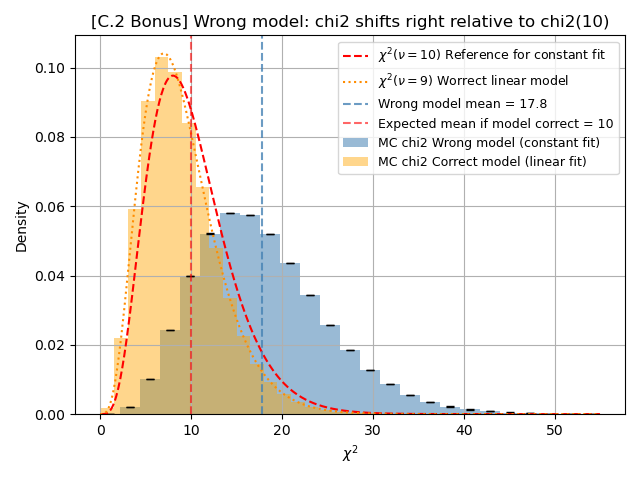
\includegraphics[width=0.65\textwidth]{fig_c2.png}
		\caption{Blue: $\chi^2$ from constant-model fits (wrong). Orange: linear-model fits (correct, from C.1). Red dashed: $\chi^2(10)$ reference. The wrong-model histogram shifts right by $\lambda \approx 7.8$, and its the blue one.} 
		\label{fig:c2}
	\end{figure}
	
\end{document}